\section{发送和接收数据}
\subsection{简述发送和接收数据}
MPTCP在发送数据方面和TCP的区别是可以从多条路径中选择一条路径来发送数据。MPTCP在接收数据方面与TCP的区别是子路径对无序包进行重排后,MPTCP的mpcb需要多所有子路径的包进行排序。二者协议栈的比较如下:
\small\begin{verbatim}
                                           +-------------------------------+
                                           |           Application         |
              +---------------+            +-------------------------------+
              |  Application  |            |             MPTCP             |
              +---------------+            + - - - - - - - + - - - - - - - +
              |      TCP      |            | Subflow (TCP) | Subflow (TCP) |
              +---------------+            +-------------------------------+
              |      IP       |            |       IP      |      IP       |
              +---------------+            +-------------------------------+
\end{verbatim}\normalsize

\subsection{数据序号映射}
由于所有的数据会通过不同的子路径发送,在接收端MPTCP需要对数据进行重新排序。因此我们需要数据序号映射。数据序号映射定义从子路径序列空间到数据序列空间的映射。子路径的序列空间是子路径自身的序列号,而数据序列空间维护着所有需发送的数据。如下图:
\begin{figure}[H]
  \centering
  % Requires \usepackage{graphicx}
  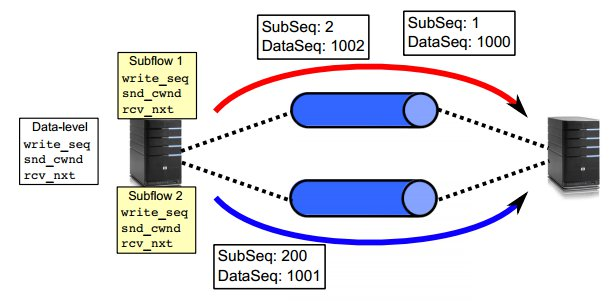
\includegraphics[width=10cm]{dias/Data-Sequence-Mapping.jpg}\\
  \caption{数据序号映射}
\end{figure}
红色子路径上的子路径序号分别是1、2,其数据序号是1000、1002。而下面的蓝色的子路径上的子路径序号和数据序号分别是200,1001。这说明从下面的蓝色子路径已经发送了199个报文,而上面的红色子路径才开始发送。在MPTCP协议定义如下:
\small\begin{verbatim}
                              1                   2                   3
              0 1 2 3 4 5 6 7 8 9 0 1 2 3 4 5 6 7 8 9 0 1 2 3 4 5 6 7 8 9 0 1
             +--------------------------------------------------------------+
             |                Data Sequence Number (8 octets)               |
             +--------------------------------------------------------------+
             |              Subflow Sequence Number (4 octets)              |
             +-------------------------------+------------------------------+
             |  Data-Level Length (2 octets) |        Zeros (2 octets)      |
             +-------------------------------+------------------------------+
\end{verbatim}\normalsize

\subsection{内核的实现}
函数mptcp\_write\_dss\_mapping对 Data Sequeue Number  和  Subflow Sequence Number进行了赋值。实现如下:
\small\begin{verbatim}
"net/mptcp/mptcp_output.c" line 318 of 1667
318 static int mptcp_write_dss_mapping(struct tcp_sock *tp, struct sk_buff *skb,
319                    __be32 *ptr)
320 {
321     struct tcp_skb_cb *tcb = TCP_SKB_CB(skb);
322     __be32 *start = ptr;
323     __u16 data_len;
324
325     *ptr++ = htonl(tcb->seq); /* data_seq */
326
327     /* If it's a non-data DATA_FIN, we set subseq to 0 (draft v7) */
328     if (mptcp_is_data_fin(skb) && skb->len == 0)
329         *ptr++ = 0; /* subseq */
330     else
331         *ptr++ = htonl(tp->write_seq - tp->mptcp->snt_isn); /* subseq */
\end{verbatim}\normalsize
第325行和331行分别对子路径序号和数据序号进行了赋值。
\small\begin{verbatim}
    data_seq and subseq
    The mapping is identify by the relative subflow seq, the data seq and
    the data len. Basically, it means that isn+sub_seq->isn+sub_seq+len at
    the subflow-level corresponds to data_seq->data_seq+len at the
    connection-level.
\end{verbatim}\normalsize
\subsection{数据接收中的重组}
内核使用三种队列接收数据,分别是:Backlog queue(sk$\rightarrow$backlog)、Prequeue queue(tp$\rightarrow$ucopy.prequeue)和 Receive queue (sk$\rightarrow$receeive\_queue)。MPTCP的实现增加了一个新的队列out-of-order queue对于各个子路径收到的数据进行重组。内核中 tcp\_v4\_rcv()的关键实现如下:
\small\begin{verbatim}
"net/ipv4/tcp_ipv4.c" line 1735 of 2581
1735     if (mptcp(tcp_sk(sk))) {
1736         meta_sk = mptcp_meta_sk(sk);
1737
1738         bh_lock_sock_nested(meta_sk);
1739         if (sock_owned_by_user(meta_sk))
1740             skb->sk = sk;
1741     } else {
1742         meta_sk = sk;
1743         bh_lock_sock_nested(sk);
1744     }
1745
1746     ret = 0;
1747     if (!sock_owned_by_user(meta_sk)) {
1748 #ifdef CONFIG_NET_DMA
1749         struct tcp_sock *tp = tcp_sk(meta_sk);
1750         if (!tp->ucopy.dma_chan && tp->ucopy.pinned_list)
1751             tp->ucopy.dma_chan = net_dma_find_channel();
1752         if (tp->ucopy.dma_chan)
1753             ret = tcp_v4_do_rcv(sk, skb);
1754         else
1755 #endif
1756         {
1757             if (!tcp_prequeue(meta_sk, skb))
1758                 ret = tcp_v4_do_rcv(sk, skb);
1759         }
1760     } else if (unlikely(sk_add_backlog(meta_sk, skb,
1761                        meta_sk->sk_rcvbuf + meta_sk->sk_sndbuf))) {
1762         bh_unlock_sock(meta_sk);
1763         NET_INC_STATS_BH(net, LINUX_MIB_TCPBACKLOGDROP);
1764         goto discard_and_relse;
1765     }
1766     bh_unlock_sock(meta_sk);
\end{verbatim}\normalsize
从第1757和1760可以看出skb只进入meta的backlog和prequeue,而和子路径的sock没有什么关系。因此,我们得出包的入队操作如下:
\begin{itemize}
  \item 进入meta\_sk的backlog
  \item 进入meta\_sk的prequeue
  \item 进入子路径的receive\_queue
\end{itemize}
第1和2种入队操作后续操作和正常TCP一致,如果是第3种情况,后续将通过函数mptcp\_queue\_skb()进入tcp\_sk(meta\_sk)$\rightarrow$out\_of\_order\_queue。{\color{red}{我觉得我研究的地方应该是这里}}
\subsection{结论}
\begin{itemize}
  \item MPTCP利用自身的Data Sequeue Number  和  Subflow Sequence Number进行了数据在各种子路径间的传输。此实现独立于TCP。
  \item 为了实现子路径的数据重组,MPTCP利用了队列out\_of\_order\_queue。
\end{itemize}